\documentclass[12pt,letterpaper, onecolumn]{exam}
\usepackage{amsmath}
\usepackage{amssymb}
\usepackage{amsfonts}
\usepackage{graphicx}
\usepackage{subcaption}
\usepackage{float}
\usepackage[shortlabels]{enumitem}
\usepackage{mathtools}
\usepackage{longtable}
\usepackage{tikz}
\usepackage{pgfplots}
\pgfplotsset{compat=1.16}
\usetikzlibrary{trees}

\usepackage[lmargin=71pt, tmargin=1.2in]{geometry} %For centering solution box
\lhead{CSC 6740 - Homework 4\\}
\rhead{Tommy Stell\\}
% \chead{\hline} % Un-comment to draw line below header
\thispagestyle{empty}   %For removing header/footer from page 1

\begin{document}

\begingroup
    \centering
    \LARGE Data Mining\\
    \LARGE Homework 4\\[0.5em]
    \large \today\\[0.5em]
    \large Tommy Stell\par

\endgroup
\noindent\rule{\textwidth}{0.4pt}
\pointsdroppedatright   %Self-explanatory
\printanswers
\renewcommand{\solutiontitle}{\noindent\textbf{Ans:}\enspace}   %Replace "Ans:" with starting keyword in solution box

\begin{questions}

    \question[20] Question 1\droppoints

    Using the data in the table to build a decision tree classifier step by step, with information gain (if your panther ID is even), GINI index (if your panther ID is odd) to classifier C0/ C1 classes. The max depth is 2.

    {\small
        \begin{longtable}{|c|c|c|c|c|}
            \hline Customer ID & Gender & Car Type & Shirt Size & Class \\ \hline
            \endhead
            \hline
            \endfoot
            1 & M & Family & Small & C0 \\
            2 & M & Sports & Medium & C0 \\
            3 & M & Sports & Medium & C0 \\
            4 & M & Sports & Large & C0 \\
            5 & M & Sports & Extra Large & C0 \\
            6 & M & Sports & Extra Large & C0 \\
            7 & F & Sports & Small & C0 \\
            8 & F & Sports & Small & C0 \\
            9 & F & Sports & Medium & C0 \\
            10 & F & Luxury & Large & C0 \\
            11 & M & Family & Large & C1 \\
            12 & M & Family & Extra Large & C1 \\
            13 & M & Family & Medium & C1 \\
            14 & M & Luxury & Extra Large & C1 \\
            15 & F & Luxury & Small & C1 \\
            16 & F & Luxury & Small & C1 \\
            17 & F & Luxury & Medium & C1 \\
            18 & F & Luxury & Medium & C1 \\
            19 & F & Luxury & Medium & C1 \\
            20 & F & Luxury & Large & C1
        \end{longtable}
        }

    \begin{solution}

        My PantherID is odd, so I will use the GINI index. For a node $t$ with class proportions $p(j\mid t)$, and a split of $n$ records into children of sizes $n_1,\dots,n_k$, we have
        \begin{equation*}
            \text{Gini}(t) = 1-\sum_{j} p(j\mid t)^2, \qquad \text{Gini}_{\text{split}} = \sum_{i=1}^{k}\frac{n_i}{n}\,\text{Gini}(i)
        \end{equation*}
        At each node we pick the attribute with the smallest $\text{Gini}_{\text{split}}$, which is the same as picking the largest drop $\Delta = \text{Gini}(\text{parent})-\text{Gini}_{\text{split}}$. I am using multiway splits on every attribute.

        I am leaving Customer ID out. Every record would land in its own leaf, giving $\text{Gini}_{\text{split}}=0$, so a blind search would pick it. It is only an identifier though, and it tells us nothing about a new customer.

        Step 1: The root node. The root has 10 C0 and 10 C1 records, so
        \begin{equation*}
            \text{Gini}(\text{root}) = 1-0.5^2-0.5^2 = 0.5
        \end{equation*}

        For Gender, the counts (C0, C1) are M: $(6,4)$ and F: $(4,6)$. Thus,
        \begin{align*}
            \text{Gini}(\text{Male})&=\text{Gini}(\text{Female})=1-0.6^2-0.4^2=0.48\\
            \text{Gini}_{\text{split}} &= \tfrac{10}{20}(0.48)+\tfrac{10}{20}(0.48) = 0.48
        \end{align*}

        For Car Type, the counts are Family: $(1,3)$, Sports: $(8,0)$ and Luxury: $(1,7)$. Thus,
        \begin{align*}
            \text{Gini}(\text{Family}) &= 1-(1/4)^2-(3/4)^2 = 0.375\\
            \text{Gini}(\text{Sports}) &= 1-1^2-0^2 = 0\\
            \text{Gini}(\text{Luxury}) &= 1-(1/8)^2-(7/8)^2 = 0.21875\\
            \text{Gini}_{\text{split}} &= \tfrac{4}{20}(0.375)+\tfrac{8}{20}(0)+\tfrac{8}{20}(0.21875) = 0.075+0.0875 = 0.1625
        \end{align*}

        For Shirt Size, the counts are Small: $(3,2)$, Medium: $(3,4)$, Large: $(2,2)$ and Extra Large: $(2,2)$. Thus,
        \begin{align*}
            \text{Gini}(\text{S}) &= 1-(3/5)^2-(2/5)^2 = 0.48\\
            \text{Gini}(\text{Med}) &= 1-(3/7)^2-(4/7)^2 = 24/49 \approx 0.4898\\
            \text{Gini}(\text{L}) &= \text{Gini}(\text{XL}) = 1-0.5^2-0.5^2 = 0.5\\
            \text{Gini}_{\text{split}} &= \tfrac{5}{20}(0.48)+\tfrac{7}{20}(0.4898)+\tfrac{4}{20}(0.5)+\tfrac{4}{20}(0.5) \approx 0.4914
        \end{align*}

        Putting these side by side,
        \begin{center}
            \begin{tabular}{|l|c|c|}
                \hline Attribute & $\text{Gini}_{\text{split}}$ & $\Delta$ \\ \hline
                Gender & 0.4800 & 0.0200 \\
                Car Type & 0.1625 & 0.3375 \\
                Shirt Size & 0.4914 & 0.0086 \\ \hline
            \end{tabular}
        \end{center}
        Car Type has the smallest $\text{Gini}_{\text{split}}$ by a wide margin, so the root splits on Car Type. The Sports branch is already pure (8 C0), so it becomes a leaf labeled C0.

        Step 2: The Family branch. This branch holds records 1, 11, 12 and 13, with counts $(1,3)$ and $\text{Gini}=0.375$.
        \begin{itemize}
            \item Gender: all four records are M, so the split has a single child identical to the parent and $\text{Gini}_{\text{split}}=0.375$. There is no gain.
            \item Shirt Size: Small $(1,0)$, Medium $(0,1)$, Large $(0,1)$ and Extra Large $(0,1)$. Every child is pure, so $\text{Gini}_{\text{split}}=0$.
        \end{itemize}
        We split on Shirt Size, with Small $\to$ C0 and Medium, Large, Extra Large $\to$ C1.

        Step 3: The Luxury branch. This branch holds records 10 and 14--20, with counts $(1,7)$ and $\text{Gini}=0.21875$.
        \begin{itemize}
            \item Gender: M is $(0,1)$ with Gini 0, and F is $(1,6)$ with Gini $1-(1/7)^2-(6/7)^2 = 12/49\approx 0.2449$. Thus,
            \begin{equation*}
                \text{Gini}_{\text{split}} = \tfrac{1}{8}(0)+\tfrac{7}{8}(0.2449) \approx 0.2143
            \end{equation*}
            \item Shirt Size: Small $(0,2)$, Medium $(0,3)$, Large $(1,1)$ and Extra Large $(0,1)$. Only Large is impure, with Gini 0.5. Thus,
            \begin{equation*}
                \text{Gini}_{\text{split}} = \tfrac{2}{8}(0)+\tfrac{3}{8}(0)+\tfrac{2}{8}(0.5)+\tfrac{1}{8}(0) = 0.125
            \end{equation*}
        \end{itemize}
        We split on Shirt Size. The Large leaf holds record 10 (C0) and record 20 (C1), which is a 1:1 tie. The tree is already at max depth 2, so it can't split any further, and I break the tie with the parent's majority class, C1.

        The final depth 2 tree is,
        \begin{center}
            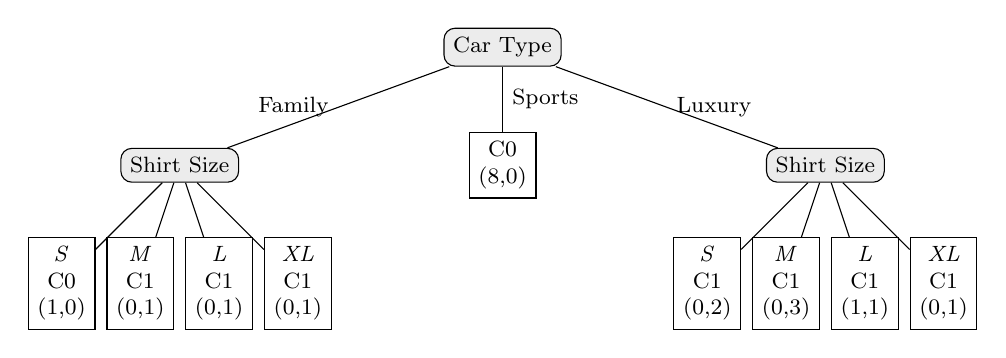
\begin{tikzpicture}[
                level distance=1.5cm,
                level 1/.style={sibling distance=4.1cm},
                level 2/.style={sibling distance=1.0cm},
                every node/.style={font=\footnotesize},
                split/.style={draw, rounded corners, fill=gray!15, align=center},
                leaf/.style={draw, align=center}
            ]
                \node[split] {Car Type}
                    child {node[split] {Shirt Size}
                        child {node[leaf] {\textit{S}\\C0\\(1,0)}}
                        child {node[leaf] {\textit{M}\\C1\\(0,1)}}
                        child {node[leaf] {\textit{L}\\C1\\(0,1)}}
                        child {node[leaf] {\textit{XL}\\C1\\(0,1)}}
                        edge from parent node[left] {Family}}
                    child {node[leaf] {C0\\(8,0)} edge from parent node[right] {Sports}}
                    child {node[split] {Shirt Size}
                        child {node[leaf] {\textit{S}\\C1\\(0,2)}}
                        child {node[leaf] {\textit{M}\\C1\\(0,3)}}
                        child {node[leaf] {\textit{L}\\C1\\(1,1)}}
                        child {node[leaf] {\textit{XL}\\C1\\(0,1)}}
                        edge from parent node[right] {Luxury}};
            \end{tikzpicture}
        \end{center}
        where each leaf shows the branch value, the predicted class, and its (C0, C1) counts. Only record 10 is misclassified, so the training error is $1/20 = 5\%$. Every Luxury leaf predicts C1, so the second split there doesn't actually change any prediction. Pruning would collapse that branch into a single C1 leaf with the same training error.

        $\square$
    \end{solution}

    \newpage
    \question[10] Question 2\droppoints

    How do you overcome the overfitting issue of the decision tree classifier? Give details how you will select the hyperparameters in practice.

    \begin{solution}

        A fully grown tree keeps splitting until every leaf is pure. Its lower levels end up fitting noise and individual records rather than real structure, so the training error keeps falling while the test error starts to climb. There are four main ways to control this, and each one has hyperparameters that need to be chosen on data the tree was not fit on.

        \begin{enumerate}[1.)]
            \item Pre-pruning (early stopping). Here we stop growing a node before it becomes pure. The hyperparameters are the maximum depth, the minimum number of records needed to split a node, the minimum number of records in a leaf, and the minimum impurity decrease (or a $\chi^2$ significance threshold) that a split has to achieve.

            To select these, I would grid-search them with $k$-fold cross-validation, usually with $k=5$ or $10$ and stratified folds when the classes are imbalanced. For example, try max depth $\in\{2,3,\dots,15\}$ and min leaf size $\in\{1,2,5,10,20,50\}$, or a fraction of $n$ such as 0.5\%--5\%. I then keep the combination with the lowest mean validation error. When two settings are within one standard error of each other, I take the simpler tree. Pre-pruning is cheap, but it can stop too early, since a split that looks useless on its own can set up a useful split below it.

            \item Post-pruning. Here we grow the full tree first, and then replace subtrees with leaves whenever that doesn't hurt the estimated generalization error. There are three common versions.
            \begin{itemize}
                \item Cost-complexity pruning. We minimize \[R_\alpha(T) = R(T)+\alpha\,|\text{leaves}(T)|,\] where $R(T)$ is the training error of tree $T$. Increasing $\alpha$ gives a nested sequence of smaller and smaller subtrees. I would pick $\alpha$ by cross-validation over that sequence, again taking the smallest tree within one standard error of the minimum.
                \item Pessimistic-error pruning. A subtree is replaced by a leaf when the upper confidence bound on the leaf's error is no worse than that of the subtree. The hyperparameter is the confidence factor (commonly 25\%), and smaller values prune more. I would tune it by cross-validation over a range such as $\{0.05, 0.10, 0.15, 0.25, 0.35\}$.
                \item Reduced-error pruning. We hold out a validation set (e.g.\ 20--30\% of the training data) and prune any node whose removal doesn't increase the error on that set. The only choice is how big the holdout is, which trades how reliable the pruning is against how much data is left to grow the tree.
            \end{itemize}

            \item Complexity penalty (minimum description length). Here we choose the tree that minimizes $\text{Cost}(\text{model})+\text{Cost}(\text{data}\mid\text{model})$, i.e.\ the training errors plus a penalty $\Omega$ for every leaf. The penalty plays the same role as $\alpha$ in cost-complexity pruning, and I would pick it the same way, by cross-validation.

            \item Ensembles. Bagging and random forests average many deep trees grown on bootstrap samples, which lowers the variance without pruning. The hyperparameters are the number of trees, the number of features tried at each split ($\sqrt{p}$ is the usual default for classification) and the leaf size. I would pick the number of trees as the point where the out-of-bag error levels off, and the features per split by out-of-bag or cross-validated error. Boosting goes the other way and combines many shallow trees. It is tuned on the number of rounds and the learning rate, using early stopping on a validation set.
        \end{enumerate}

        In every case, the final test set stays untouched during tuning and is used once at the very end to report the error of the chosen model. If that reported number has to be unbiased as well, the tuning goes inside an inner cross-validation loop that runs separately within each outer training fold (nested cross-validation).

        $\square$
    \end{solution}

    \newpage
    \question[20] Question 3\droppoints

    Use the Naive Bayes classifier to predict the new data as positive or negative class, using the Laplace estimate to avoid the zero-probability condition. New data: $[A=1, B=0, C=0]$. Which class? Show the step-by-step procedure.

    {\small
    \begin{longtable}{|c|c|c|c|c|}
        \hline Record & A & B & C & Class \\ \hline
        \endhead
        \hline
        \endfoot
        1 & 0 & 0 & 0 & + \\
        2 & 0 & 0 & 1 & - \\
        3 & 0 & 1 & 1 & - \\
        4 & 0 & 1 & 1 & - \\
        5 & 0 & 0 & 1 & + \\
        6 & 1 & 0 & 1 & + \\
        7 & 1 & 0 & 1 & - \\
        8 & 1 & 0 & 1 & - \\
        9 & 1 & 1 & 1 & + \\
        10 & 1 & 0 & 1 & +
    \end{longtable}
    }

    \begin{solution}

        Naive Bayes assumes the attributes are conditionally independent given the class, and assigns $X=(A=1,B=0,C=0)$ to the class that maximizes
        \begin{equation*}
            P(c\mid X) \propto P(c)\,P(A=1\mid c)\,P(B=0\mid c)\,P(C=0\mid c)
        \end{equation*}

        Step 1: The priors. Class $+$ holds records 1, 5, 6, 9, 10 and class $-$ holds records 2, 3, 4, 7, 8, so $n_+ = n_- = 5$ and
        \begin{equation*}
            P(+) = P(-) = \tfrac{5}{10} = 0.5
        \end{equation*}
        Smoothing the prior as well would give $(5+1)/(10+2) = 0.5$, so it makes no difference here.

        Step 2: The raw counts.
        \begin{center}
            \begin{tabular}{|c|c|c|}
                \hline & Class $+$ ($n=5$) & Class $-$ ($n=5$) \\ \hline
                $\#(A=1)$ & 3 & 2 \\
                $\#(B=0)$ & 4 & 3 \\
                $\#(C=0)$ & 1 & 0 \\ \hline
            \end{tabular}
        \end{center}
        Every class $-$ record has $C=1$, so the unsmoothed estimate is $P(C=0\mid -) = 0/5 = 0$. That one zero would force $P(-\mid X)=0$ no matter what the other attributes say, which is exactly the zero-probability problem.

        Step 3: The Laplace estimate. Each attribute is binary ($k=2$ values), so we add 1 to every count and 2 to every denominator,
        \begin{equation*}
            P(x_i\mid c) = \frac{n_{c,x_i}+1}{n_c+k} = \frac{n_{c,x_i}+1}{5+2}
        \end{equation*}
        which gives,
        \begin{center}
            \begin{tabular}{|c|c|c|}
                \hline & Class $+$ & Class $-$ \\ \hline
                $P(A=1\mid c)$ & $(3+1)/7 = 4/7$ & $(2+1)/7 = 3/7$ \\
                $P(B=0\mid c)$ & $(4+1)/7 = 5/7$ & $(3+1)/7 = 4/7$ \\
                $P(C=0\mid c)$ & $(1+1)/7 = 2/7$ & $(0+1)/7 = 1/7$ \\ \hline
            \end{tabular}
        \end{center}

        Step 4: The class scores.
        \begin{align*}
            P(X\mid +)P(+) &= \tfrac{4}{7}\cdot\tfrac{5}{7}\cdot\tfrac{2}{7}\cdot 0.5 = \tfrac{40}{343}\cdot 0.5 \approx 0.1166\cdot 0.5 = 0.0583\\
            P(X\mid -)P(-) &= \tfrac{3}{7}\cdot\tfrac{4}{7}\cdot\tfrac{1}{7}\cdot 0.5 = \tfrac{12}{343}\cdot 0.5 \approx 0.0350\cdot 0.5 = 0.0175
        \end{align*}

        Step 5: The decision. Since $0.0583 > 0.0175$, the new record is classified as positive ($+$). Normalizing the two scores gives
        \begin{equation*}
            P(+\mid X) = \frac{40}{40+12} = \frac{10}{13} \approx 0.769, \qquad P(-\mid X) = \frac{3}{13}\approx 0.231
        \end{equation*}

        $\square$
    \end{solution}

    \newpage
    \question[30] Question 4\droppoints

    A manufacturing company wants to automatically classify finished units as good or bad quality. Two analysts have each built a classifier from the same historical inspection data of 1,000 records (850 good, 150 bad):
    \begin{itemize}
        \item Analyst A built a decision tree (C4.5-style, with pessimistic-error pruning).
        \item Analyst B built a naive Bayes classifier (with Laplace smoothing).
    \end{itemize}

    Your task is to design a fair comparison of the two classifiers and determine, using the results below, whether one performs significantly better than the other. Treat bad as the positive class throughout.

    Table 1. Error rates (\%) from stratified 10-fold cross-validation. Both classifiers used the same folds; each test fold has 100 records (85 good, 15 bad).
    {\small
        \begin{longtable}{|l|c|c|c|c|c|c|c|c|c|c|}
            \hline Fold & 1 & 2 & 3 & 4 & 5 & 6 & 7 & 8 & 9 & 10 \\ \hline
            \endhead
            \hline
            \endfoot
            Decision Tree & 12 & 14 & 11 & 15 & 13 & 12 & 16 & 13 & 12 & 14 \\
            Naive Bayes & 14 & 15 & 14 & 14 & 15 & 12 & 19 & 14 & 14 & 15
        \end{longtable}
        }

    Table 2. Confusion matrices pooled over all 10 test folds ($n = 1{,}000$).
    {\small
        \begin{longtable}{|l|c|c|c|c|}
            \hline  & \shortstack{DT: predicted\\bad} & \shortstack{DT: predicted\\good} & \shortstack{NB: predicted\\bad} & \shortstack{NB: predicted\\good} \\ \hline
            \endhead
            \hline
            \endfoot
            Actually Bad & 105 & 45 & 126 & 24 \\
            Actually Good & 87 & 763 &  122 & 728
        \end{longtable}
        }
        \begin{enumerate}[1.]
            \item Analyst A reports that the decision tree reached 98$\%$ accuracy on the data it was trained on. Explain why this number can't be used to compare the classifiers.
            \item Explain why the cross-validation should be stratified for this dataset, and why both classifiers must be evaluated on the same folds for paired-t-test.
            \item Both analysts tuned hyperparameters (the pruning confidence factor and the smoothing strength). Describe a procedure that tunes them without biasing the error estimates, and name the problem your procedure prevents.
            \item From Table 2, compute for each classifier: accuracy, error rate, precision, recall (sensitivity), specificity and F1 for the bad class. Present the results in a table.
            \item Using Table 1, carry out a paired t-test at $\alpha = 0.05$ on the per-fold differences in error rate. State H$_0$ and H$_1$, compute t statistic, give the degrees of freedom and the critical value, and state your conclusion.
        \end{enumerate}

    \newpage
    \begin{solution}

        \begin{enumerate}[1.]
            \item The 98\% is the resubstitution (training) accuracy. It measures how well the tree memorized the records it was built from, not how it will do on new units, so it is optimistically biased. A decision tree can push its training error toward 0 just by growing deeper, which means this number mostly reflects how complex the tree is. It also isn't a like-for-like comparison, since there is no matching training figure for naive Bayes, and a flexible model like a tree gets inflated far more by training accuracy than a rigid model like naive Bayes. From Table 2, the cross-validated accuracy for the same learner is $(105+763)/1000 = 86.8\%$, more than 11 points lower. Accuracy is also a weak yardstick here, since predicting ``good'' for every unit already scores $850/1000 = 85\%$ while catching none of the bad units. The only fair comparison is error measured on held-out data, using the same folds for both models.

            \item Bad units are only 15\% of the data. With purely random folds of 100 records, the number of bad units in a fold would change by chance. It is roughly binomial with mean 15 and standard deviation $\sqrt{100\cdot 0.15\cdot 0.85}\approx 3.6$, so some folds could easily hold 8 bad units and others 22 (about $\pm 2$ standard deviations). That adds variance to the per-fold error, precision and recall, and could leave a training split short on the minority class. Stratified folds keep the 85/15 ratio in every fold, so each fold estimate comes from the same class mix the model will see in deployment, and the fold-to-fold variance reflects the classifiers rather than the split.

            The paired t-test works on the differences $d_i = \text{err}_{NB,i}-\text{err}_{DT,i}$, which only mean something if both errors in a pair come from the same training and test records. Some folds are simply harder than others (fold 7 is the worst fold for both models), so the two error series move together. From Table 1, the sample variances are $s^2_{DT} = 2.4$ and $s^2_{NB}\approx 3.16$, and the sample covariance is $\widehat{\operatorname{Cov}}\approx 1.98$, a correlation of $r\approx 0.72$. Pairing cancels this shared fold difficulty, since
            \begin{align*}
                \operatorname{Var}(d_i) &= \operatorname{Var}(\text{err}_{NB})+\operatorname{Var}(\text{err}_{DT})-2\operatorname{Cov}(\text{err}_{NB},\text{err}_{DT})\\
                &= 2.4+3.16-2(1.98) = 1.6
            \end{align*}
            which is much smaller than either variance on its own. If we ignored the pairing and ran an unpaired two-sample test on the same numbers, we would get
            \begin{equation*}
                t = \frac{14.6-13.2}{\sqrt{2.4/10+3.16/10}}\approx 1.88 < t_{0.025,\,18} = 2.101,
            \end{equation*}
            and we would fail to reject. The pairing is what makes the difference detectable. With different folds there is no natural pairing, the covariance term is lost, and the paired test is invalid.

            \item I would use nested cross-validation. The outer loop is the stratified 10-fold split that produces the reported error. Inside each outer training set of 900 records, I would run a separate inner stratified $k$-fold CV (e.g.\ 5-fold) over a grid of the pruning confidence factor (e.g.\ $0.05$--$0.5$) for the tree and of the smoothing pseudo-count (e.g.\ $0.1$--$10$) for naive Bayes. The value with the lowest inner CV error is chosen, the model is refit on all 900 records, and it is evaluated once on the 100-record outer test fold. This way the outer test fold never influences the choice of hyperparameters. Both models get the same tuning budget and the same outer folds, so their errors stay paired. A simpler alternative is to set aside a separate validation split for tuning and keep a final test set that is used only once.

            The problem this prevents is optimistic selection bias, i.e.\ test-set leakage or overfitting the model selection. If the hyperparameters were chosen by looking at the same folds used to report the error, the reported error would be the minimum over many tries. That understates the true error, and it understates it more for whichever model had the larger search grid, which biases the comparison.

            \item With bad as the positive class, $TP$ is actual bad predicted bad, $FN$ is actual bad predicted good, $FP$ is actual good predicted bad, and $TN$ is actual good predicted good. Reading these off Table 2,
            \begin{center}
                {\small
                \begin{tabular}{|l|c|c|}
                    \hline & Decision tree & Naive Bayes \\ \hline
                    $TP,\ FN,\ FP,\ TN$ & $105,\ 45,\ 87,\ 763$ & $126,\ 24,\ 122,\ 728$ \\ \hline
                    Accuracy $=\frac{TP+TN}{n}$ & $868/1000 = 0.868$ & $854/1000 = 0.854$ \\
                    Error rate $=\frac{FP+FN}{n}$ & $132/1000 = 0.132$ & $146/1000 = 0.146$ \\
                    Precision $=\frac{TP}{TP+FP}$ & $105/192 = 0.547$ & $126/248 = 0.508$ \\
                    Recall $=\frac{TP}{TP+FN}$ & $105/150 = 0.700$ & $126/150 = 0.840$ \\
                    Specificity $=\frac{TN}{TN+FP}$ & $763/850 = 0.898$ & $728/850 = 0.856$ \\
                    $F_1 = \frac{2\,TP}{2\,TP+FP+FN}$ & $210/342 = 0.614$ & $252/398 = 0.633$ \\ \hline
                \end{tabular}
                }
            \end{center}
            As a check, the pooled error rates match the averages of the per-fold errors in Table 1, $132/10 = 13.2\%$ and $146/10 = 14.6\%$. The decision tree has the higher accuracy, precision and specificity. Naive Bayes catches 21 more bad units (recall $0.84$ vs.\ $0.70$) and has the higher $F_1$, at the cost of 35 more false alarms. Which one is better in practice depends on whether shipping a bad unit costs more than rejecting a good one.

            \item Let $d_i = \text{err}_{NB,i}-\text{err}_{DT,i}$ in percentage points, with $k=10$ folds. The hypotheses are
            \begin{align*}
                H_0&: \mu_d = 0 \quad \text{(the two classifiers have the same true error rate)}\\
                H_1&: \mu_d \neq 0 \quad \text{(their error rates differ)}
            \end{align*}
            so the test is two-sided. From Table 1,
            \begin{center}
                {\small
                \begin{tabular}{|c|c|c|c|c|c|c|c|c|c|c|}
                    \hline Fold & 1 & 2 & 3 & 4 & 5 & 6 & 7 & 8 & 9 & 10 \\ \hline
                    $d_i$ & 2 & 1 & 3 & $-1$ & 2 & 0 & 3 & 1 & 2 & 1 \\
                    $d_i-\bar d$ & 0.6 & $-0.4$ & 1.6 & $-2.4$ & 0.6 & $-1.4$ & 1.6 & $-0.4$ & 0.6 & $-0.4$ \\
                    $(d_i-\bar d)^2$ & 0.36 & 0.16 & 2.56 & 5.76 & 0.36 & 1.96 & 2.56 & 0.16 & 0.36 & 0.16 \\ \hline
                \end{tabular}
                }
            \end{center}
            and thus,
            \begin{align*}
                \bar d &= \tfrac{1}{10}\textstyle\sum d_i = \tfrac{14}{10} = 1.4\\
                s_d^2 &= \tfrac{1}{k-1}\textstyle\sum (d_i-\bar d)^2 = \tfrac{14.4}{9} = 1.6, \qquad s_d = \sqrt{1.6}\approx 1.265\\
                t &= \frac{\bar d}{s_d/\sqrt{k}} = \frac{1.4}{1.265/\sqrt{10}} = \frac{1.4}{0.4} = 3.5
            \end{align*}
            The degrees of freedom are $k-1 = 9$. From the t table (row df $=9$, two-tails $0.05$ column, $t_{.975}$), the critical value is $t_{0.025,\,9} = 2.262$.

            Since $|t| = 3.5 > 2.262$, we reject $H_0$ at $\alpha=0.05$. The exact two-sided p-value is $p\approx 0.0067$, which sits between the $0.01$ and $0.002$ two-tail columns of the table ($3.250 < 3.5 < 4.297$). The decision tree's cross-validated error rate is about 1.4 percentage points lower than naive Bayes's, with a 95\% confidence interval of $1.4 \pm 2.262\times 0.4 = [0.50,\ 2.30]$. This conclusion is only about the overall error rate. On the bad class itself, naive Bayes catches more of the bad units (126 of 150 against 105 for the tree), so which model is ``better'' depends on the cost of missing a bad unit.

            One caveat is that the ten training sets overlap (any two share 800 of their 900 records), so the $d_i$ are not truly independent and the plain paired test is somewhat liberal. A common correction inflates the variance factor from $\tfrac{1}{k}$ to $\tfrac{1}{k}+\tfrac{n_{\text{test}}}{n_{\text{train}}} = 0.1+\tfrac{100}{900}\approx 0.211$, which gives $t = 1.4/\sqrt{0.211\times 1.6}\approx 2.41 > 2.262$ ($p\approx 0.039$). So the conclusion still holds, just with less margin.
        \end{enumerate}

        $\square$
    \end{solution}

    \newpage
    \question[10] Question 5\droppoints

    The data tuples of the table below are sorted by decreasing probability value, as returned by a classifier, of being classified as positive. We test a list of thresholds used to make the final positive/negative calls. The threshold list is [0.4, 0.50, 0.55, 0.6, 0.65, 0.7, 0.8, 0.9]; data tuples with Prob. $\geq$ Threshold will be Positive, otherwise Negative.

    {\small
        \begin{longtable}{|c|c|c|}
            \hline Tuple & Class (True) & Prob. (Model) \\ \hline
            \endhead
            \hline
            \endfoot
            1 & p & 0.95 \\
            2 & n & 0.85 \\
            3 & p & 0.78 \\
            4 & p & 0.66 \\
            5 & n & 0.60 \\
            6 & p & 0.55 \\
            7 & n & 0.53 \\
            8 & n & 0.52 \\
            9 & n & 0.51 \\
            10 & p & 0.40
        \end{longtable}
        }

        \begin{enumerate}[a.)]
            \item Find TP, FP, TN, FN, and Sensitivity (TP Rate: TPR), Specificity (TN Rate: TNR), and False Positive Rate (FPR: 1-TNR) for each threshold.
            \item Fill in the table.
            \item Draw the ROC curve and compute AUC.
        \end{enumerate}

    \begin{solution}

        There are $P=5$ positive tuples (1, 3, 4, 6, 10) and $N=5$ negative tuples (2, 5, 7, 8, 9). At each threshold, every tuple with Prob.\ $\geq$ threshold is called positive, and
        \begin{equation*}
            TPR = \frac{TP}{P},\qquad TNR = \frac{TN}{N},\qquad FPR = \frac{FP}{N} = 1-TNR
        \end{equation*}

        a.) and b.) Going down the list one threshold at a time, the filled-in table is,

            {\small
            \begin{longtable}{|c|c|c|c|c|c|c|c|c|}
                \hline Threshold & Called positive & TP & FP & TN & FN & TPR & TNR & FPR \\ \hline
                \endhead
                \hline
                \endfoot
                0.90 & 1 & 1 & 0 & 5 & 4 & 0.2 & 1.0 & 0.0 \\
                0.80 & 1--2 & 1 & 1 & 4 & 4 & 0.2 & 0.8 & 0.2 \\
                0.70 & 1--3 & 2 & 1 & 4 & 3 & 0.4 & 0.8 & 0.2 \\
                0.65 & 1--4 & 3 & 1 & 4 & 2 & 0.6 & 0.8 & 0.2 \\
                0.60 & 1--5 & 3 & 2 & 3 & 2 & 0.6 & 0.6 & 0.4 \\
                0.55 & 1--6 & 4 & 2 & 3 & 1 & 0.8 & 0.6 & 0.4 \\
                0.50 & 1--9 & 4 & 5 & 0 & 1 & 0.8 & 0.0 & 1.0 \\
                0.40 & 1--10 & 5 & 5 & 0 & 0 & 1.0 & 0.0 & 1.0
            \end{longtable}
            }

            c.) The ROC curve plots $(FPR, TPR)$ for each threshold. I also add the point $(0,0)$, which corresponds to a threshold above 0.95 where nothing is called positive.
            \begin{center}
                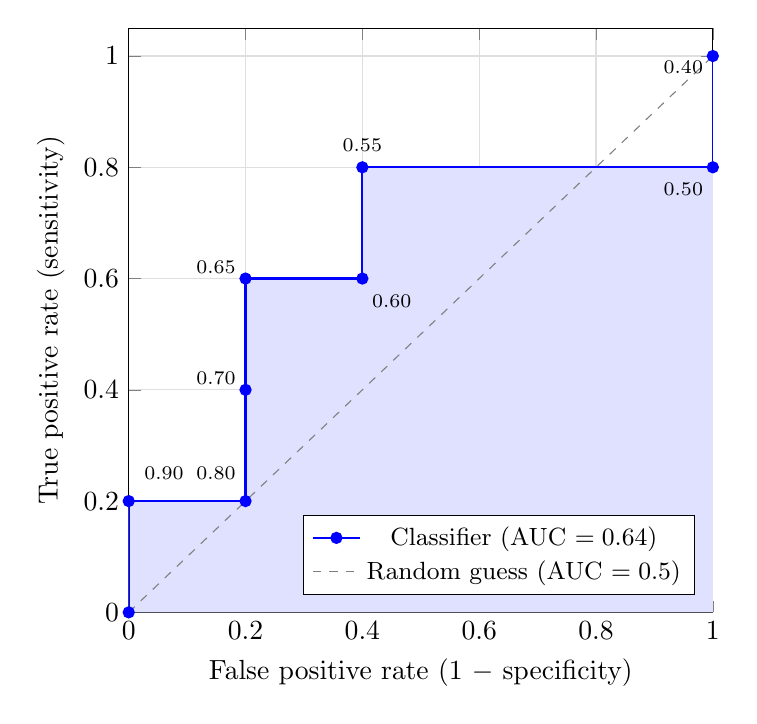
\begin{tikzpicture}
                    \begin{axis}[
                        width=9cm, height=9cm,
                        xmin=0, xmax=1, ymin=0, ymax=1.05,
                        xlabel={False positive rate (1 $-$ specificity)},
                        ylabel={True positive rate (sensitivity)},
                        xtick={0,0.2,0.4,0.6,0.8,1}, ytick={0,0.2,0.4,0.6,0.8,1},
                        grid=major, grid style={gray!25},
                        legend pos=south east, legend style={font=\small}
                    ]
                        \addplot[fill=blue!12, draw=none, forget plot] coordinates {
                            (0,0) (0,0.2) (0.2,0.2) (0.2,0.4) (0.2,0.6) (0.4,0.6) (0.4,0.8) (1,0.8) (1,1) (1,0)
                        } \closedcycle;
                        \addplot[thick, blue, mark=*, mark size=1.8pt] coordinates {
                            (0,0) (0,0.2) (0.2,0.2) (0.2,0.4) (0.2,0.6) (0.4,0.6) (0.4,0.8) (1,0.8) (1,1)
                        };
                        \addlegendentry{Classifier (AUC $=0.64$)}
                        \addplot[dashed, gray] coordinates {(0,0) (1,1)};
                        \addlegendentry{Random guess (AUC $=0.5$)}
                        \node[font=\scriptsize, anchor=west] at (axis cs:0.01,0.25) {0.90};
                        \node[font=\scriptsize, anchor=east] at (axis cs:0.2,0.25) {0.80};
                        \node[font=\scriptsize, anchor=east] at (axis cs:0.2,0.42) {0.70};
                        \node[font=\scriptsize, anchor=east] at (axis cs:0.2,0.62) {0.65};
                        \node[font=\scriptsize, anchor=west] at (axis cs:0.4,0.56) {0.60};
                        \node[font=\scriptsize, anchor=south] at (axis cs:0.4,0.81) {0.55};
                        \node[font=\scriptsize, anchor=east] at (axis cs:1,0.76) {0.50};
                        \node[font=\scriptsize, anchor=east] at (axis cs:1,0.98) {0.40};
                    \end{axis}
                \end{tikzpicture}
            \end{center}

            The curve is a step function, so the area under it is just a sum of rectangles. The trapezoid rule gives the same answer, since every segment of the curve is either vertical or horizontal. Thus,
            \begin{align*}
                \text{AUC} &= \underbrace{(0.2-0)(0.2)}_{FPR\in[0,0.2]} + \underbrace{(0.4-0.2)(0.6)}_{FPR\in[0.2,0.4]} + \underbrace{(1-0.4)(0.8)}_{FPR\in[0.4,1]}\\
                &= 0.04 + 0.12 + 0.48 = 0.64
            \end{align*}
            As a check, the AUC is also the probability that a randomly chosen positive is scored above a randomly chosen negative. Counting the positive--negative pairs that are ranked correctly, tuple 1 beats all 5 negatives, tuples 3 and 4 beat 4 each (all but tuple 2), tuple 6 beats 3 (tuples 7, 8, 9), and tuple 10 beats none. That gives
            \begin{equation*}
                \frac{5+4+4+3+0}{5\cdot 5} = \frac{16}{25} = 0.64
            \end{equation*}
            The classifier does better than random guessing (0.5), but not by much, mostly because positive tuple 10 is scored below every negative.

        $\square$
    \end{solution}

    \newpage
    \question[10] Question 6\droppoints

    Describe the Adaboost algorithm using decision tree as a base classifier.

    \begin{solution}

        AdaBoost builds a sequence of $T$ small decision trees, usually stumps (depth 1) or trees only a few levels deep. Each new tree focuses on the training records that the earlier trees got wrong, and the final prediction is a weighted vote of all the trees. We start with $n$ training records.

        Step 1: Initialize the weights. Every record starts with the same weight, $w_j = 1/n$ for $j=1,\dots,n$.

        Step 2: Train a tree on the weighted data. In round $t$, fit a shallow tree using the current weights. The weights can either go straight into the Gini (or entropy) calculation, or we can draw a new training set of $n$ records with replacement, where record $j$ is picked with probability $w_j$. The depth is kept small so that each tree is a weak learner and doesn't overfit.

        Step 3: Compute the weighted error. The error of the tree is the total weight of the records it gets wrong,
        \begin{equation*}
            \varepsilon_t = \sum_{\text{misclassified } j} w_j
        \end{equation*}
        Since the weights add up to 1, $\varepsilon_t$ is between 0 and 1. If $\varepsilon_t > 0.5$, the tree is doing worse than random guessing, so we throw it out, reset every weight to $1/n$, and redo the round. If $\varepsilon_t = 0$, the tree is already perfect and we can stop.

        Step 4: Compute the tree's vote weight.
        \begin{equation*}
            \alpha_t = \frac{1}{2}\ln\left(\frac{1-\varepsilon_t}{\varepsilon_t}\right)
        \end{equation*}
        A tree with a small error gets a large $\alpha_t$, and a tree with an error near 0.5 gets an $\alpha_t$ near 0, so more accurate trees get a bigger say in the final vote.

        Step 5: Update the record weights. Records the tree got wrong become heavier, and records it got right become lighter,
        \begin{align*}
            w_j &\leftarrow w_j\, e^{\alpha_t} \quad \text{if record } j \text{ was misclassified}\\
            w_j &\leftarrow w_j\, e^{-\alpha_t} \quad \text{if record } j \text{ was classified correctly}
        \end{align*}
        Then we divide every weight by the new total so the weights add up to 1 again. After this step the misclassified records hold exactly half of the total weight, so the next tree is pushed to get them right.

        Step 6: Repeat. Go back to Step 2 until all $T$ trees are built. $T$ is chosen by cross-validation, or by stopping once the error on a validation set stops improving.

        Step 7: Classify a new record. Each tree votes for the class it predicts, and its vote counts $\alpha_t$. We add up the votes for each class, and the class with the largest total wins.

        Since the trees are shallow, boosting mainly reduces bias. Because it keeps upweighting the hard records, it can be sensitive to noisy labels and outliers.

        $\square$
    \end{solution}

\end{questions}
\end{document}
